\documentclass[a4paper,12pt]{article}
\usepackage[ngerman]{babel}
\usepackage{ucs}
\usepackage{multirow}
\usepackage{xltxtra}
\usepackage[utf8x]{inputenc}
\usepackage{fontspec}
\usepackage{eurosym}
\usepackage{graphicx}
\usepackage[paper=a4paper,left=25mm,right=25mm,top=25mm,bottom=25mm]{geometry}
\usepackage{makecell}
\usepackage[table]{xcolor}
\usepackage{float}
\usepackage[normalem]{ulem}
\usepackage{xcolor,colortbl}
\definecolor{Gray}{gray}{0.85}
\usepackage[automark]{scrlayer-scrpage}
\setlength{\parindent}{0em}
\setlength{\parskip}{1ex}
\pagestyle{scrheadings}
\clearscrheadfoot
\setmainfont[Mapping=tex-text]{Liberation Serif}
\begin{document}
\input{theme.tex}
\input{version.tex}
\ohead{Regelstand: \commitDate, id: \commitID}
\title{\tagYear\ a-MAZE-ing Challenge Regeln}

\makeatletter
\let\inserttitle\@title
\makeatother
\begin{center}
	\rrgerLogo
	\huge                      % Schriftgröße einstellen
	\bfseries                   % Fettdruck einschalten
	\\
	\inserttitle
\end{center}
\section{Ziel}
Entwerfe, baue und programmiere einen Roboter, der einem erhöhten Holzlabyrinth
folgen kann, ohne herunterzufallen. Das Abschließen des Labyrinths vor dem
Zeitlimit erhöht Deine Punktzahl um Bonuspunkte.

\section{Altersgruppen}
Die Teams, die an dieser Challenge teilnehmen, treten in den Altersgruppen
Grundschule (ES) und Mittelstufe (MS) an. (Hinweis: Wenn in einer der beiden
Divisionen weniger als 5 Teams angemeldet sind, hat der Veranstaltungsleiter
die Möglichkeit, die Altersgruppen zu kombinieren)

\section{Roboter}
Autonomer Roboter, basierend auf beliebiger Plattform, der \euro{1.500}  oder
weniger kostet und die folgenden Designbedingungen erfüllt, die beim Check-In
überprüft werden:
\begin{itemize}
	\item Der Roboter darf keine externen Sensoren verwenden, die ihm
		helfen, dem Labyrinth zu folgen; jedoch sind Drehgeber (Motor
		Encoder) erlaubt.
	\item Das Volumen des Roboters darf 65030 cm$^{3}$ nicht überschreiten.
\end{itemize}

\section{Allgemeine Spiel- und Punktregeln}
\begin{itemize}
	\item Der Veranstalter legt die Anzahl der erlaubten offiziellen Läufe
		fest und die Anzahl dieser offiziellen Läufe, die für die
		Gesamtpunktzahl gezählt werden, die zur Ermittlung der
		Top-8-Teams, die an dem Turnier teilnehmen werden, verwendet
		wird.
	\item Der Roboter hat 2 Minuten Zeit, um das Labyrinth abzuschließen,
		wobei die Uhr von 120 Sekunden rückwärts läuft.
	\item Die Teams können nach Bedarf üben, wobei sie sich mit anderen
		übenden Teams abwechseln. Sollte die Bahn für einen offiziellen
		Lauf benötigt werden, geben die Übungsteams die Bahn ab.
	\item Jede abgeschlossene Gerade ist 50 Punkte wert. Eine Gerade gilt
		als abgeschlossen, wenn ein beliebiger Teil des Roboters über
		den Beginn der Markierungslinie der Wertungszone fährt.
	\item Jeder abgeschlossene Winkel ist 100 Punkte wert. Ein Winkel gilt
		als abgeschlossen, wenn ein beliebiger Teil des Roboters über
		den Beginn der Markierungslinie der Wertungszone fährt.
	\item Wenn der Roboter aus dem Labyrinth fällt, bevor er die Ziellinie
		erreicht hat, und noch Zeit übrig ist, bringe ihn zur
		Startlinie zurück und versuche, das Labyrinth zu beenden.
	\item Ein Roboter gilt als aus dem Labyrinth gefallen, wenn eines
		seiner Räder die Oberfläche des Labyrinths \textbf{VOLLSTÄNDIG}
		nicht mehr berührt.
	\item Wenn der Roboter das Labyrinth nach Ablauf der Zeit nicht
		beendet, entspricht der Punktestand demjenigen zurückgelegten
		Abschnitt der Strecke, der am weitesten vom Start entfernt ist.
	\item Wenn der Roboter das Labyrinth vor Ablauf der Zeit fertigstellt,
		entspricht die Punktzahl der maximalen Punktzahl für seine
		Altersgruppe, zuzüglich eines Bonus, bestehend aus 1 Punkt für
		jede verbleibende Sekunde.
\end{itemize}

\section{Spielfeld Spezifikation}
\begin{itemize}
	\item Alle a-MAZE-ing Strecken werden so nah wie möglich an der
		Zeichnung sein und aus Leimholz (oder einem ähnlichen lokal
		beschafften Material) von 24 cm Breite und 2 cm Höhe gebaut. Es
		gibt verschiedene Längen mit Kombinationen von 45, 90 und 135
		Grad Kurven in beide Richtungen. (Anmerkung: Alle Challenge
		Maße sind ungefähre Angaben).
\end{itemize}
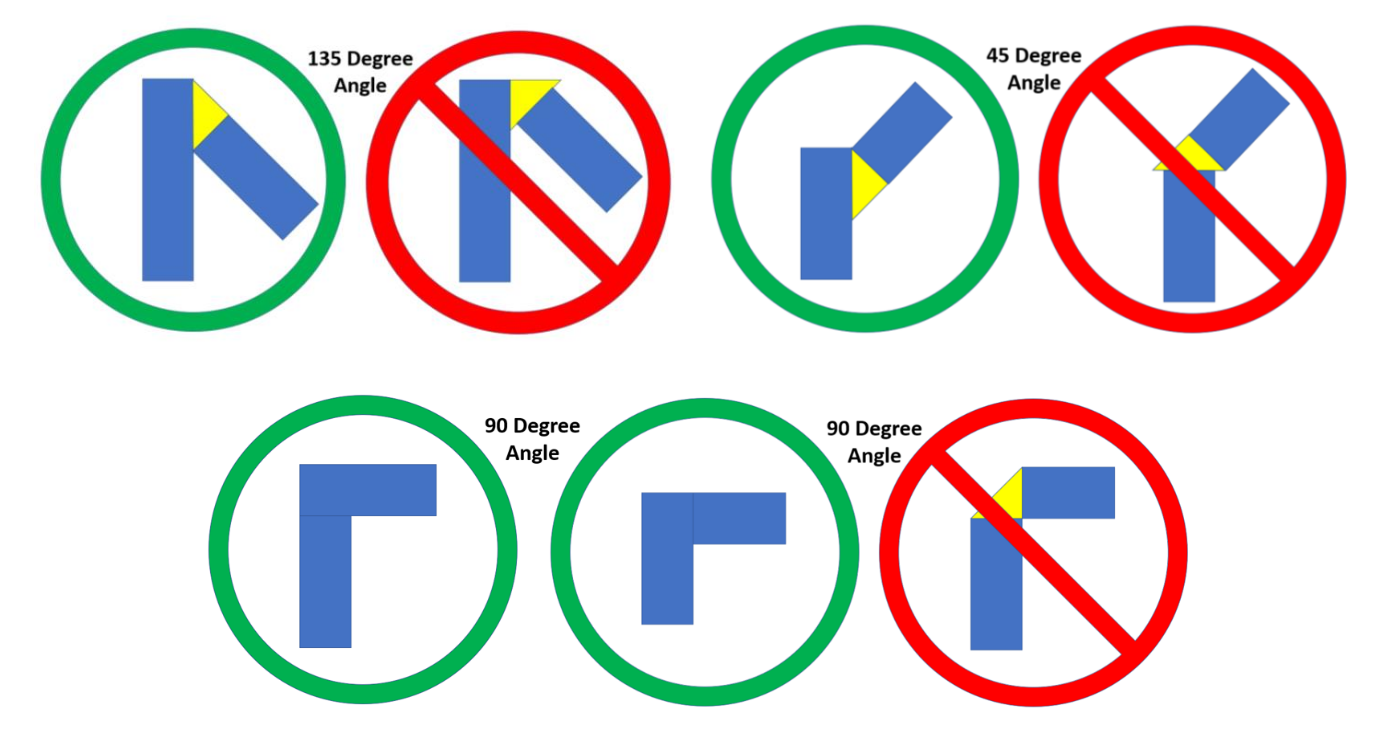
\includegraphics[width=1.0\textwidth]{amazeing_allowed.png}
\begin{itemize}
	\item Die Teile werden normalerweise mit starkem Gewebeklebeband
		zusammengeklebt. Sie können jedoch auch mit Schrauben oder
		geklebten Verzahnungen verbunden werden. Unabhängig von der
		verwendeten Methode werden alle erforderlichen Maßnahmen
		ergriffen, um sicherzustellen, dass die Schienen so glatt und
		frei von Unregelmäßigkeiten wie möglich sind.
	\item In der Altersgruppe ES gibt es 4 Geraden und 3 Kurven was
		insgesamt 500 Punkte ermöglich.
	\item In der Altersgruppe MS gibt es 6 Geraden und 5 Kurven was
		insgesamt 800 Punkte ermöglich.
	\item Abhängig vom Veranstaltungsraum und dem verfügbaren Material
		können beide Altersgruppe auf der längeren MS-Strecke betrieben
		werden. In diesem Fall befindet sich die Ziellinie der
		Altersgruppe ES irgendwo zwischen der 3. und 4. abgewinkelten
		Kurve der MS-Bahn.
	\item Wertungslinien:
		\begin{enumerate}
			\item Das folgende Diagramm zeigt die Platzierung der
				Bewertungslinien für jeden der drei
				Winkeltypen.
			\item Start und Ziel sind markiert
			\item Die Wertungslinien am Ende jeder Geraden und
				jeder Kurve sind mit den auf der Fahrt vom
				Start bis zum Ziel akkumulierten Punkten
				beschriftet (dies vereinfacht die Überwachung
				der Punkte).
				\begin{center}
					\begin{tabular}{|c|c|c|c|c|c|} \hline
						\rowcolor{Gray}
						1. Gerade & 1. Kurve & 2. Gerade & 2. Kurve & 3. Gerade & 3. Kurve  \\ \hline
						50 & 150 & 200 & 300 & 350 & 450  \\ \hline
						\rowcolor{Gray}
						4. Gerade & 4. Kurve & 5. Gerade & 5. Kurve & 6. Gerade & \\ \hline
						500 (ES Ziel) & 600 & 650 & 750 & 800 (MS Ziel) & \\ \hline
					\end{tabular}
				\end{center}
		\end{enumerate}
		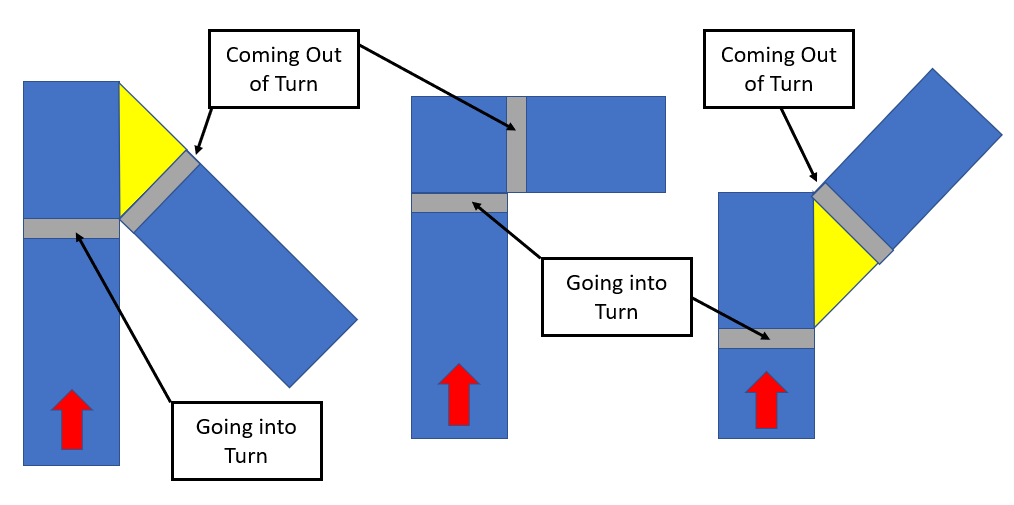
\includegraphics[width=1.0\textwidth]{amazeing_angle.png}
\end{itemize}

\section{Turnierplan}
\begin{itemize}
	\item Die besten 8 Mannschaften jeder Altersklasse treten in einem
		Turnier gegeneinander an.
	\item Gleichstand wird auf der Grundlage eines vom Veranstalter
		gewählten LEISTUNGSKRITERIUMS aufgelöst. (Zum Beispiel: die
		höchste Einzelwertung aller gleichwertigen Mannschaften).
	\item Die aufsteigenden Teams werden entsprechend ihrer Gesamtpunktzahl
		in die Turnierklasse gesetzt (siehe untenstehende Tabelle).
		\begin{figure}[H]
			\centering
			\def\svgwidth{\columnwidth}
			\input{tournament_score/tournament_score.pdf_tex}
		\end{figure}
	\item Der zweite Platz ("`Runner Up"') wird verwendet, um den 3. Platz
		auf der Grundlage des Ergebnisses der Halbfinalrunde zu
		bestimmen.
\end{itemize}
\end{document}
